\documentclass[a4paper,10pt]{report}
\usepackage{anysize} % Soporte para el comando \marginsize
\marginsize{1.2cm}{1.2cm}{1cm}{1cm}
\usepackage{amsfonts}
\usepackage{amssymb}
\usepackage{mathpazo}
\usepackage[latin1]{inputenc}
\usepackage[english,spanish]{babel}
\usepackage{amsmath}
\usepackage{multicol} 
\columnsep=7mm
\usepackage{latexsym}
\usepackage{mathrsfs}
\usepackage{indentfirst}
\usepackage{graphicx}
\usepackage{enumitem}

\usepackage{times}

\setlength{\paperwidth}{216mm} \setlength{\paperheight}{219mm}
\setlength{\textwidth}{39pc} \setlength{\textheight}{58.5pc}
\setlength{\topmargin}{-1cm} \setlength{\oddsidemargin}{-0.5cm}
\setlength{\evensidemargin}{-0.9cm}

\newcommand{\ds}{\displaystyle}
\newcommand{\normal}{\triangleleft \,}
\newcommand{\tx}{\textrm}

\newcommand{\Z}{\mathbb{Z}}
\newcommand{\N}{\mathbb{N}}
\newcommand{\R}{\mathbb{R}}
\newcommand{\e}{\rightarrow}
\newcommand{\bi}{\Leftrightarrow}
\newcommand{\com}{\mathbb{N} \bi}
\newcommand{\fu}{f:\N \e \R}
\newcommand{\ba}{\backslash}
\newcommand{\Q}{\mathbb{Q}}

\newcommand{\calP}{\mathcal{P}}
\newcommand{\calF}{\mathcal{F}}
\newcommand{\calL}{\mathcal{L}}

\newcommand{\ovl}{\overline}
\newcommand{\ora}{\overrightarrow}
\newcommand{\ola}{\overleftarrow}
\newcommand{\olra}{\overleftrightarrow}
\newcommand{\ula}{\underleftarrow}
\newcommand{\ura}{\underrightarrow}

\newcommand{\inner}[2]{\langle{#1},{#2}\rangle}

\newcommand{\cabecera}[1]{\begin{figure}[h]
 \begin{minipage}[c]{0.05\columnwidth}
\centering
\includegraphics[width=2cm]{escudo.pdf}
\end{minipage}
\hfill{}
\begin{minipage}[c]{0.86\columnwidth}
\centering\flushleft {Universidad Nacional de Ingenier\'ia\\
Facultad de Ciencias\\
Escuela Profesional de Matem\'atica \hfill #1}
\end{minipage}
\end{figure}\vspace{-0.5cm}
}


\pagestyle{empty}
\begin{document}
\cabecera{Ciclo 2018 - II}

\begin{center}
{\Large \textbf{Pr\'actica dirigida de C\'alculo de Probabilidades}}\\
{\Large \textbf{CM-	1H2}}
\end{center}

\noindent
\rule{\textwidth}{0.6pt}

\vspace{0.5cm}

\textbf{Probabilidad condicional, eventos independientes}

\begin{enumerate}
\item  Para cualquier colecci\'on finita de eventos $A_1,\cdots,A_n$, prueba que
$$\mathbb{P}(A_1\cap\cdots\cap A_n)=\mathbb{P}(A_1)P(A_2|A_1)\cdots \mathbb{P}(A_n|A_1\cap\cdots\cap A_{n-1})$$
siempre que $\mathbb{P}(A_1\cap\cdots\cap A_n)>0$.

\item Consideremos las familias que tienen dos ni\~nos y supongamos que varones y mujeres son igualmente
probables. Si escogemos al azar una familia y en ella hay un hijo var\'on, ?`cu\'al es la probabilidad de que el otro hijo sea tambi\'en var\'on?. Luego, considera de nuevo las familias que tienen dos hijos.
Si escogemos un ni\~no al azar entre estas familias y resulta ser var\'on, ?`cu\'al es la probabilidad de que el otro ni\~no en la familia tambi\'en sea var\'on?.
\item Prueba que si $\mathbb{P}(A) = a$ y $\mathbb{P}(B) = b$  entonces  $\mathbb{P}(A|B) \geq  (a + b -1)/b$.
\item En una bolsa se colocan $n$ tarjetas con nombres escritos en ellas y se extraen dos, sucesivamente
y sin reposici\'on. Si $m < n$ de los nombres son de mujer, calcula la probabilidad de que el segundo
nombre extra\'ido sea de mujer.
\item Un caminante sale del punto o y escoge uno de los caminos $ob_1$, $ob_2$, $ob_3$, $ob_4$ al azar. En cada uno de los cruces siguientes de nuevo escoge al azar. ?`Cu\'al es la probabilidad de que
el caminante llegue al punto a?.
\begin{center}
	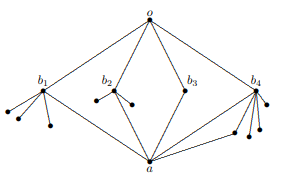
\includegraphics[scale=1]{G1.png}
\end{center}
\item Cada vez que el repartidor de una pizzeria regresa a buscar los pedidos para repartir, se encuentra que pueden haber entre 1 y 5 encargos esperando, y cada una de estas posibilidades tiene la misma probabilidad. Si, en promedio, la mitad de los clientes le da propina, calcule la probabilidad de que obtenga al menos dos propinas en un viaje.

\item Se selecciona aleatoriamente un n\'umero del conjunto $\{1, 2,\dots, 10.000\}$ y se observa que es impar. ?`Cu\'al es la probabilidad de que sea  divisible por $3$  y  que no sea divisible por $3$ y $5$?.
\item En una escuela internacional, $60$ estudiantes, de los cuales $15$ son coreanos, $20$ son franceses, $8$ son griegos y el resto son chinos, se dividen al azar en cuatro clases de $15$ estudiantes  cada una. Si hay un total de ocho estudiantes franceses y seis coreanos en las clases $A$ y $B$. ?`Cu\'al es la probabilidad de que la clase $C$ tenga $4$ de los $12$ restantes estudiantes  franceses y $3$ de los restantes $9$ estudiantes coreanos?.
\item En una comunidad de $M$ hombres y $w$ mujeres, $m$ hombres y $w$ mujeres fuman ($m \leq M , w \leq W $). Si una persona es seleccionada al azar y $A$ y $B$ son los eventos que indican que una  persona es  hombre y fuma, respectivamente.?` Bajo que condiciones  $A$ y $B$ son independientes?.
\item Prueba que si $A$, $B$ y $C$ son independientes, entonces $A$ y $B \cap B$ son independientes. Muestra que $A -B$ y $C$ son independientes.

\end{enumerate}
\vspace{0.5cm}

\textbf{Ley de probabilidad total, teorema de Bayes}

\begin{enumerate}
\item Tres enfermedades distintas y excluyentes $A$, $B$ y $C$ producen el mismo conjunto de s\'intomas $H$. Un estudio cl\'inico muestra que las probabilidades de contraer las enfermedades son $0.01$; $0.005$ y $0.02$ respectivamente. Adem\'as, la probabilidad de que el paciente desarrolle los s\'intomas $H$ para cada enfermedad son $0.90$; $0.95$ y $0.75$, respectivamente. Si una persona enferma tiene los s\'intomas $H$, ?`cu\'al es la probabilidad de que tenga la enfermedad $A$?.
\item Un estudiante responde una pregunta de un examen de m\'ultiple selecci\'on que tiene cuatro respuestas posibles. Suponga que la probabilidad de que el estudiante conozca la respuesta a la pregunta es $0.8$ y la probabilidad de que adivine es $0.2$. Si el estudiante adivina, la probabilidad de que acierte es $0.25$. Si el estudiante responde acertadamente la pregunta, ?`cu\'al es la probabilidad de que el estudiante realmente supiera la respuesta?.
\item El primer hijo que tiene una mujer es un ni\~no hemof\'ilico. La mujer, en cuya historia familiar
no aparecen casos de hemofilia, tiene dudas sobre tener un segundo hijo, pero piensa que su hijo
no hered\'o la hemofilia de ella y que su enfermedad es debida a una mutaci\'on. Por lo tanto, la
probabilidad de que un segundo hijo tenga hemofilia es la de que nuevamente la enfermedad venga de una mutaci\'on, y esto es un n\'umero peque\~no, $m$ (digamos $m=10^{-5}$). Calcula cu\'al es en realidad la probabilidad de que el segundo hijo tenga hemofilia si el primero naci\'o hemof\'ilico.
\item Supongamos que existen $N$ familias en la tierra y que el n\'umero m\'aximo de hijos de una familia es $c$. Sea $\alpha_j (0 \leq j \leq c, \displaystyle \sum_{j = 0}^c \alpha_j = 1)$ la fracci\'on de familias con $j$ ni\~nos. Encuentra la fracci\'on de todos los ni\~nos en el mundo que son los k-nacidos  de sus familias ($k =1, 2,\dots, c$).
\item Hay dos establos en una granja, uno que contiene $20$ caballos y $13$ mulas, el otro con $25$ caballos y ocho mulas. Los animalitos  de vez en cuando dejan sus establos y luego regresan a sus establos. Supongamos que durante un periodo en que todos los animalitos est\'an en sus establos, un caballo sale de un establo y luego regresa. ?` Cu\'al es la probabilidad de que el siguiente animalito que salga del mismo establo sea tambi\'en un caballo?.
\item Una urna contiene cinco chips rojos y tres azules. Supongamos que cuatro de estos chips son seleccionados al azar y transferidos a una segunda urna, que originalmente estaba vac\'ia. Si un chip aleatorio de esta segunda urna es azul. ?`Cu\'al es la probabilidad de que dos chips rojos y dos azules fueran transferidos de la primera urna a la segunda?.

\item Supongamos que el $80\%$ de los estudiantes de \'ultimo a\~no, el $70\%$ de los estudiantes de tercer a\~no, el $50\%$ de los estudiantes de segundo a\~no y el $30\%$ de los estudiantes de primer a\~o de una universidad utilizan con frecuencia la biblioteca de su campus. Si el $30\%$ de todos los estudiantes son estudiantes de primer a\~no, el $25\%$ son estudiantes de segundo a\~no, el $25\%$ son estudiantes de tercer a\~no y el $20\%$ son personas de \'ultimo a\~no, ?`qu\'e porcentaje de todos los estudiantes usan la biblioteca con frecuencia?.

\item Un juez est\'a $65\%$ seguro de que un sospechoso ha cometido un crimen. Durante el transcurso del juicio, un testigo convence al juez de que hay un $85\%$ de posibilidades de que el criminal sea zurdo. Si el $23\%$ de la poblaci\'on es zurda y el sospechoso tambi\'en es zurdo, con esta nueva informaci\'on, ?`cu\'an seguro deber\'ia ser el juez de la culpabilidad del sospechoso?.

\item La ventaja de un cierto an\'alisis de sangre es que el $90\%$ de veces es positivo para los pacientes que tienen una cierta enfermedad. Su desventaja es que el $25\%$ de las veces tambi\'en es positivo en personas sanas. En un cierto lugar el $30\%$ de la gente tiene la enfermedad y cualquier persona con una prueba de sangre positiva se le da un medicamento que cure la enfermedad. Si el $20\%$ de veces el medicamento produce escocedura. ?`Cu\'al es la probabilidad de que una persona de este lugar que tiene escocedura tuvo la enfermedad en primer lugar?.

\item En un estudio realizado hace tres a\~nos, se encontr\'o que el $82\%$ de las personas en una muestra seleccionada al azar ten\'ia calificaciones crediticias financieras "buenas", mientras que el $18\%$ restante ten\'ia calificaciones crediticias financieras "malas". Los registros actuales de las personas de esa muestra muestran que el $30\%$ de aquellos con malas calificaciones crediticias han mejorado sus calificaciones desde entonces, mientras que el $15\%$ de aquellos con buenas calificaciones crediticias han cambiado desde entonces a tener una mala calificaci\'on de cr\'edito. ?`Qu\'e porcentaje de personas con buenas calificaciones crediticias ahora, ten\'ian malas calificaciones hace tres a\~nos?.

\end{enumerate}
\vspace{0.5cm}

\textbf{Variables aleatorias, funci\'on de masa de probabilidad, funci\'on de distribuci\'on acumulativa}

\vspace{0.3cm}

\begin{enumerate}
\item Sea X una variable aleatoria con funci\'on de masa probabilidad dada por la siguiente tabla:
\begin{center}
	\begin{tabular}{cccccccccc}
		$x_i$  &:& -2& -1& 0 &1& 2& 3& 4& 5\\
		$\pi$ &:& 0.1& 0.2& 0.15& 0.2& 0.1& 0.15& 0.05& 0.05
	\end{tabular}
\end{center}
Calcula las probabilidades de los siguientes eventos:
\begin{itemize}
	\item $X$ es negativa
	\item $X$ es par
	\item $X$ toma valores entre 1 y 5, ambos inclusive.
	\item $\mathbb{P}(X = -2|X \leq 0)$
	\item $\mathbb{P}(X \geq 2|X > 0)$.
\end{itemize}
\item Dos dados  son lanzados y el valor absoluto de la diferencia de los resultados se denota por $X$.

?` Cu\'ales son los valores posibles de $X$ y las probabilidades asociadas con esos valores?.

\item De una urna que contiene $5$ chips rojos, $5$ blancos y $5$  azules,  sacamos dos chips al azar. Por cada chip azul ganamos $1$ sol , por cada chip blanco ganamos $2$ soles, pero por cada chip rojo perdemos  $3$ soles. Si $X$ representa la cantidad que ganamos o perdemos. ?`Cu\'ales son los posibles valores de $X$ y las probabilidades asociadas a eso valores?.

\item En una sociedad de poblaci\'on $N$, la probabilidad es  $p$  que una persona tenga cierta enfermedad  independientemente de otras. Sea $X$ el n\'umero de personas que deben ser examinadas hasta que se encuentre una persona con la enfermedad, $X = 0$ si no se encuentra a nadie con la enfermedad. 

?` Cu\'ales son los posibles valores de X?. Determina las probabilidades asociadas con estos valores.
\item Determina el valor de la constante A para que las siguientes sean funciones de masa de probabilidad.
\begin{itemize}
	\item $ \mathbb{P}(X = i) = \left\{\begin{matrix}
	A_i& i = 1, 2,\cdots , n\\
	0 & \text{en otro caso}.
	\end{matrix} \right.$		
	\item $\mathbb{P}(X = i) = \left\{\begin{matrix}
	A_i/2^i& i = 1, 2,\cdots , n\\
	0 & \text{en otro caso}.
	\end{matrix} \right.$
	\item $\mathbb{P}(X = i) = \left\{\begin{matrix}
	A_i/3^i& i = 1, 3,\cdots , 2n-1\\
	A_i/4^i& i = 2, 4,\cdots , 2n\\
	0 & \text{en otro caso}.
	\end{matrix} \right.$
\end{itemize}
\item En lanzamientos  sucesivos de un dado justo, sea $X$ el n\'umero de lanzamientos hasta que aparezca el primer $6$. Determine la funci\'on de masa de probabilidad y la funci\'on de distribuci\'on de  $X$.

\item Un dado  se lanza sucesivamente. Sea $X$ el n\'umero de lanzamientos hasta que cada uno de los seis posibles resultados ocurran al menos una vez. Encuentra la funci\'on de masa de probabilidad de $X$.

\item En una ciudad hay $40$ taxis, numerados del  $1$ al  $40$. Tres taxis llegan al azar a  una estaci\'on para recoger pasajeros. ?` Cu\'al es la probabilidad de que el n\'umero de al menos uno de los taxis sea menor de 5?.

\item En el experimento de lanzar un dado equilibrado dos veces, sea X el m\'aximo de los dos n\'umeros obtenidos. Determina y dibuja la funci\'on de masa de probabilidad y la funci\'on de distribuci\'on de X.
\item Sea X la cantidad de nacimientos en un hospital hasta que nazca la primera ni\~na. Determina la funci\'on de masa de probabilidad y la funci\'on de distribuci\'on de X. Suponga que la probabilidad es 1/2 de que un beb\'e nacido sea una ni\~na.
\end{enumerate}

\vspace{0.5cm}

\textbf{Esperanza matem\'atica}
\begin{enumerate}
\item Demuestra que si $X \geq 0$ y existe $\mathbb{E}(X)$, entonces $\mathbb{E}(X) \geq 0$.
\item Demuestra que si  $X$ es una variable aleatoria acotada entonces existe $\mathbb{E}(X)$.
\item Proporciona una variable aleatoria discreta, para la cual no exista valor esperado.
\item Sean X una variable aleatoria discreta y $g : \mathbb{R}\to\mathbb{R}$ una funci\'on y consideremos la nueva variable aleatoria discreta $Y=g(X)$. Prueba que, si existe la esperanza matem\'atica de $Y$, \'esta es $\displaystyle \mathbb{E}[Y]=\sum_{n=1}^{\infty}g(x_n)p_n$.
\item Un dado  se lanza sucesivamente. Sea $X$ el n\'umero de lanzamientos hasta que cada uno de los seis posibles resultados ocurran al menos una vez. Encuentra la funci\'on de masa de probabilidad de $X$.

\item Lanzamos  una moneda  dos veces y sea  $X$  el n\'umero de caras obtenidas. ?` Cu\'al es la esperanza o el valor esperado  de X?.
\item Escribimos los n\'umeros $a_1, a_2, \dots $ , para  bolas id\'enticas y las mezclamos  en una caja. ?`Cu\'al es el valor esperado de una bola seleccionada al azar?.
\item En la loteria de un determinado estado, los jugadores eligen seis enteros diferentes entre el $1$ y $49$, siendo el orden de selecci\'on irrelevante. La comisi\'on de la loteria entonces selecciona seis de estos n\'umeros al azar como los n\'umeros que deberian ser los ganadores. Un jugador gana el gran premio de $1,200,000$ soles, si los seis n\'umeros que ha seleccionado coinciden con los n\'umeros ganadores. Gana el segundo y tercer premio de $800$ y $35$ soles, respectivamente, si exactamente cinco y cuatro de sus seis n\'umeros seleccionados coinciden con los n\'umeros ganadores. ?` Cu\'al es la  esperanza  de la cantidad que un jugador gana en un juego?.

\item La funci\'on distribuci\'on de una variable aleatoria $X$ es dado por:

\[
F(x) = \begin{cases}
0 & \ x < -3 \\
3/8 & \ -3 \leq x < 0 \\
1/2 & \ 0 \leq x < 3 \\
3/4 & \ 3 \leq x < 4 \\
1 & \ x \geq 4
\end{cases}
\]

Calcula $\mathbb{E}(X), \mathbb{E}(X^2 - 2\vert X \vert )$ y $\mathbb{E}(X\vert X \vert)$.
 \item Proporciona  un ejemplo de dos variables aleatorias X e Y que no sean independientes, pero que, sin embargo,
$\mathbb{E}(XY ) = \mathbb{E}(X) \mathbb{E}(Y )$, lo cual implica que no est\'an correlacionadas.
\end{enumerate}
\end{document}